\begin{itemize}
    \item \textbf{Contract Funding}: In this phase, Alice broadcasts her Contract Funding transaction. Then Bob will do the same and the Temp transaction will be broadcast whether by Bob or Erin. Now, all other contract funding transactions will be broadcast. If anybody does not follow the protocol, everything will be reverted by not revealing the \Aone key. Otherwise, Alice will reveal the \Aone key by broadcasting Erin's Margin Deposit transaction. Then other funding transactions will be broadcast. Then Bob will broadcast the Temp transaction. If Bob does not, Erin will.

    \item \textbf{Principal Deposition}: Now it is the time for principal deposition. The first one who deposits his principal must be Bob due to the value of locktimes on the Default transactions. If someone does not deposit his principal, the Arbitrage will meet the same fate as previous types of Arbitrage, and Alice will take the ownership of Erin's margin while other parties, except the one who actually defaults on his margin, exchange their margins with their previous party. In this phase, the genesis swaption is on its Delay Keeper stage. By the end of Erin's principal deposition, the Payback transaction will be broadcasted. In the default case, instead of the Payback transaction, the Time's Up transaction will be used. The Payback transaction also needs to be double-colored border with Alice's and Erin's colors.
    
    \item \textbf{Leader Lock}: Like the considerations mentioned in {\it Unsecured Bond} section we take care of Erin's assets as well here. If Bob tries to cheat even after Alice's payback deposition (Which is supposed to be fulfilled by Erin's money), she will broadcast Bob Anti-Cheat and get Bob's principal as punishment besides taking back Erin's principal. If Alice and Bob cooperatively try to cheat on Erin by neither broadcasting Bob Anti-Cheat nor revealing the \keyone key, Erin to prevent his money to be blocked can broadcast Alice Bob Anti-Cheat transaction and take his money back.
    
    \item \textbf{Option Contract}: This is time for Alice to use her option. Since in all swptions the right-hand side party is in charge of revealing \Atwo key, all locktimes need to be descending which is not possible due to the loop structure of the arbitrage. To solve this problem, we delegate the option to Bob. So, in this stage, if Alice lets her option expire, the option is delegated to Bob. 
    
    \item \textbf{Option Delegation}: In this phase, the option is Bob's and every one is waiting for him. If he exercises the option, every one gets their new coins, otherwise every one gets their old coins. Note  that  if  Alice  has  decided  not  to exercise, Bob would also not exercise. Since if  it was not beneficial for Alice it  would not be beneficial for Bob neither. the reason is that the coins that Alice gets are the same as Bob gets, so if one has lost its value the other one has lost too.
\end{itemize}

\begin{figure*}[!ht]
    \centering
    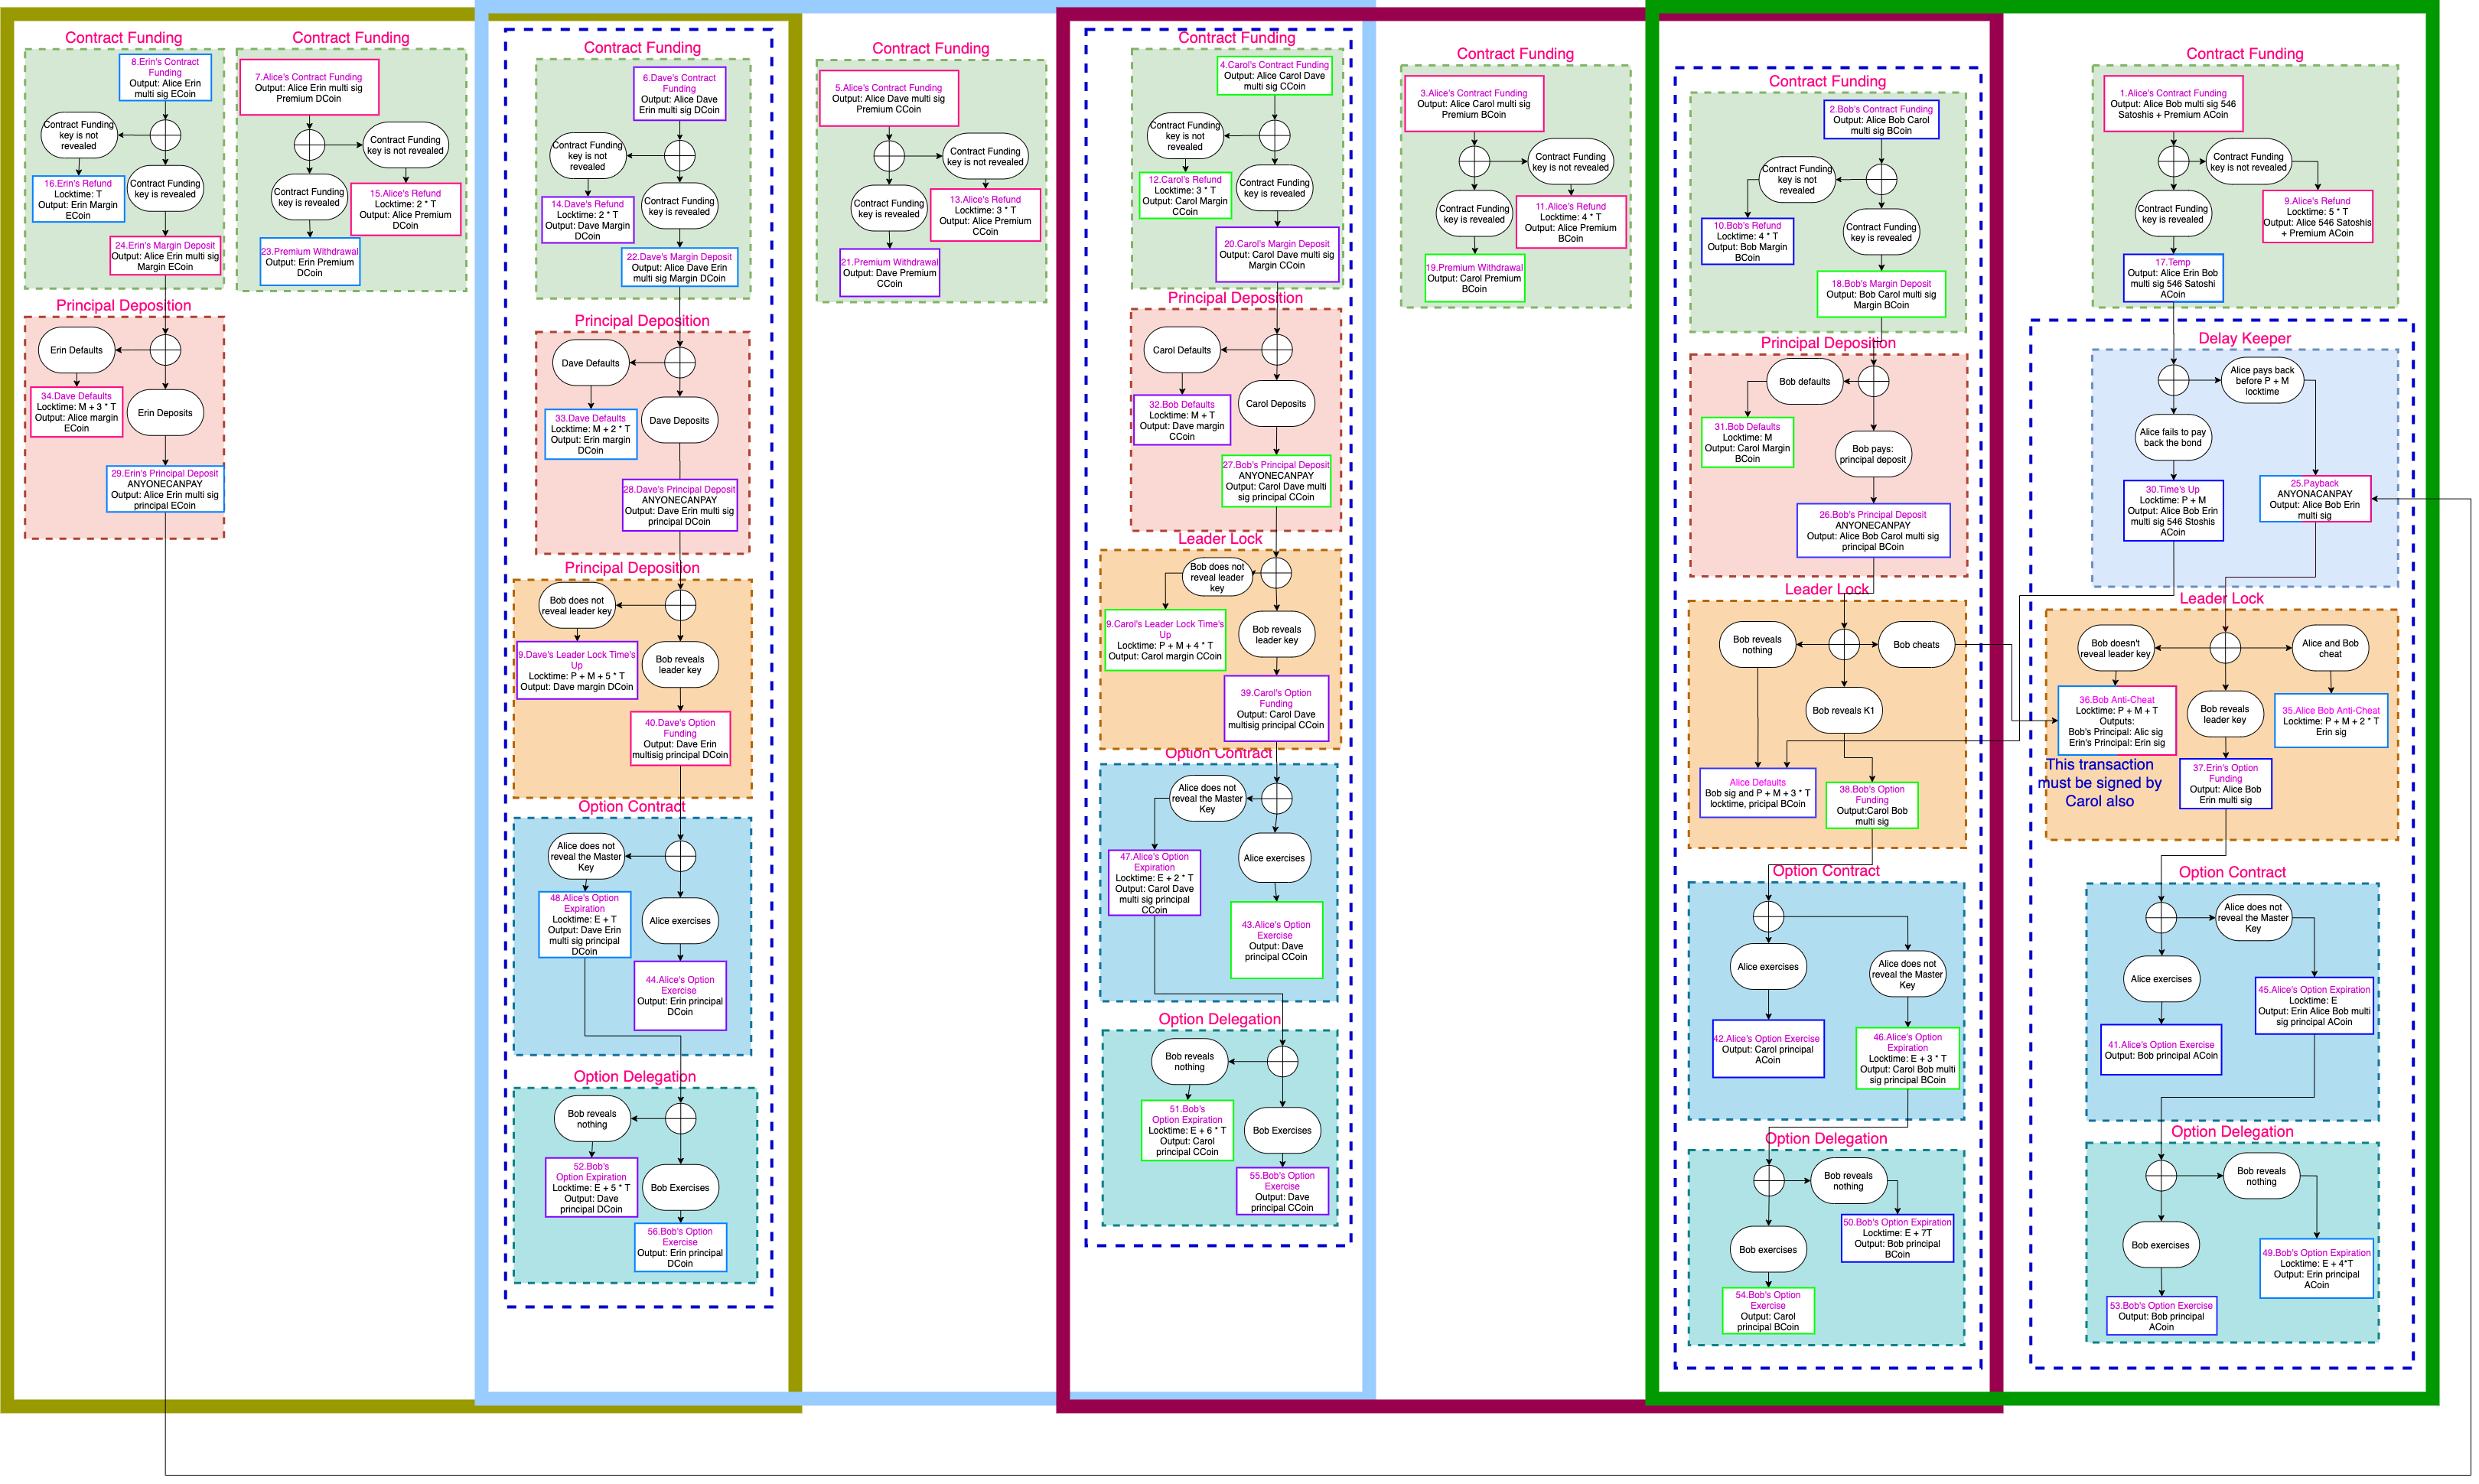
\includegraphics[width=\textwidth]{figures/bond-initiated-arbitrage.png}
    \caption{The Bond-Initiated Arbitrage. Pink-bordered transactions are broadcast by Alice, blue-bordered ones by Bob, green-bordered ones by Carol, purple-bordered ones by Dave, light blue ones by Erin and the double-color-bordered ones can be broadcast by either parties.}
    \label{fig:bond-arbitrage}
\end{figure*}